\documentclass[listings]{labreport}
\usepackage{amsmath}
\subject{Теория автоматов}
\titleparts{Практическое задание №1}{Вариант 8}
\students{Лабушев Тимофей}
\usepackage{caption}
\captionsetup{justification=raggedright, singlelinecheck=false}

\begin{document}

\maketitlepage

\section*{Цель работы}

Практическое освоение методов взаимного преобразования автоматных моделей Мили и Мура.
Проверка абстрактных автоматов Мили и Мура на эквивалентность.

\section*{Задание}

\begin{enumerate}
\item В соответствии с выбранным номером варианта осуществить преобразование автомата Мили в автомат Мура.
\item Сформировать входное слово необходимой длины. Длина входного слова должна быть минимальна,
  но достаточна для осуществления всех имеющихся в графах автоматов переходов.
\item Используя сформированное входное слово, осуществить проверку исходного и полученного в результате
  преобразования автоматов на эквивалентность. В качестве исходного состояния выбрать состояние $а_1$.
\item Далее осуществить преобразование полученного на предыдущем этапе автомата Мура в автомат Мили.
\item Сформировать входное слово необходимой длины. Длина входного слова должна быть минимальна,
  но достаточна для осуществления всех имеющихся в графах автоматов переходов.
\item Используя сформированное входное слово, осуществить проверку исходного и полученного в результате
  преобразования автоматов на эквивалентность. В качестве исходного состояния выбрать состояние $a_1$.
\end{enumerate}

\section*{Исходный автомат Мили}

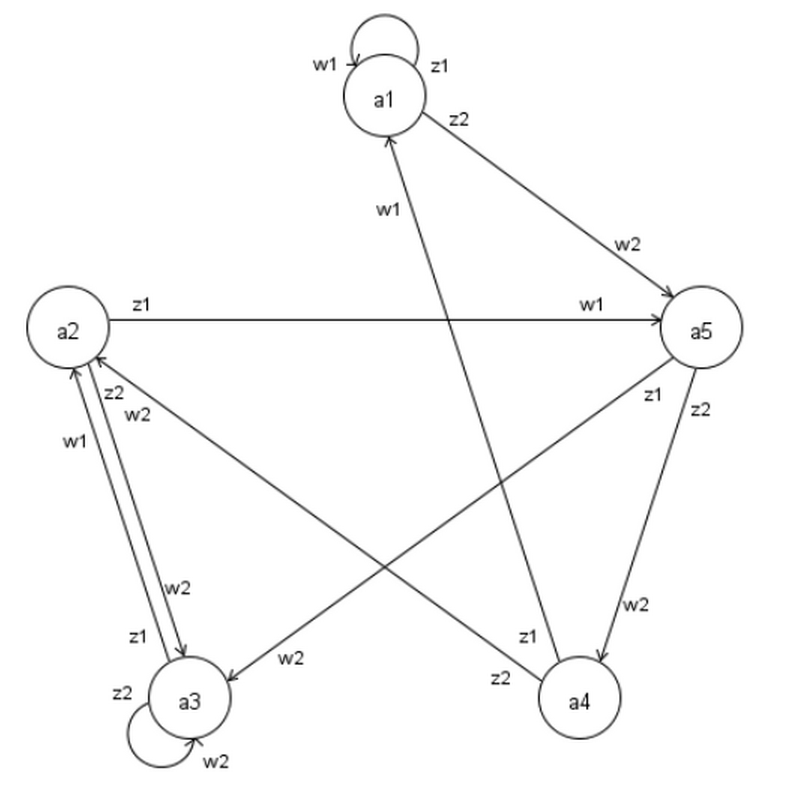
\includegraphics[width=0.6\textwidth]{HW1.png}

\subsection*{Входное слово}

\begin{table}[h]
\begin{tabular}{|c|c|c|c|c|c|c|c|c|c|c|c|c|c|}
\hline
$z_1$ & $z_2$ & $z_1$ & $z_2$ & $z_1$ & $z_2$ & $z_1$ & $z_1$ & $z_2$ & $z_1$ & $z_2$ & $z_2$ & $z_2$ & \\\hline

$a_1$ & $a_1$ & $a_5$ & $a_3$ & $a_3$ & $a_2$ & $a_3$ & $a_2$ & $a_5$ & $a_4$ & $a_1$ & $a_5$ & $a_4$ & $a_2$ \\\hline

$w_1$ & $w_2$ & $w_2$ & $w_2$ & $w_1$ & $w_2$ & $w_1$ & $w_1$ & $w_2$ & $w_1$ & $w_2$ & $w_2$ & $w_2$ & \\\hline
\end{tabular}
\caption{Поведение исходного автомата}
\end{table}

\section*{Преобразование в автомат Мура}

Поставим каждому состоянию автомата Мили в соответствие множество всевозможных
пар $a_s w_g$, где $a_s$ — функция $\delta$ от состояния и входного сигнала,
$w_g$ — функция $\lambda$ от состояния и входного сигнала.
Каждую полученную пару возьмем за состояние $b_s$ преобразованного автомата.

$$a_1: a_1w_1 = b_1$$
$$a_2:
\begin{cases}
a_2w_1 = b_2 \\
a_2w_2 = b_3
\end{cases}$$
$$a_3: a_3w_2 = b_4$$
$$a_4: a_4w_2 = b_5$$
$$a_5:
\begin{cases}
a_5w_1 = b_6 \\
a_5w_2 = b_7
\end{cases}$$

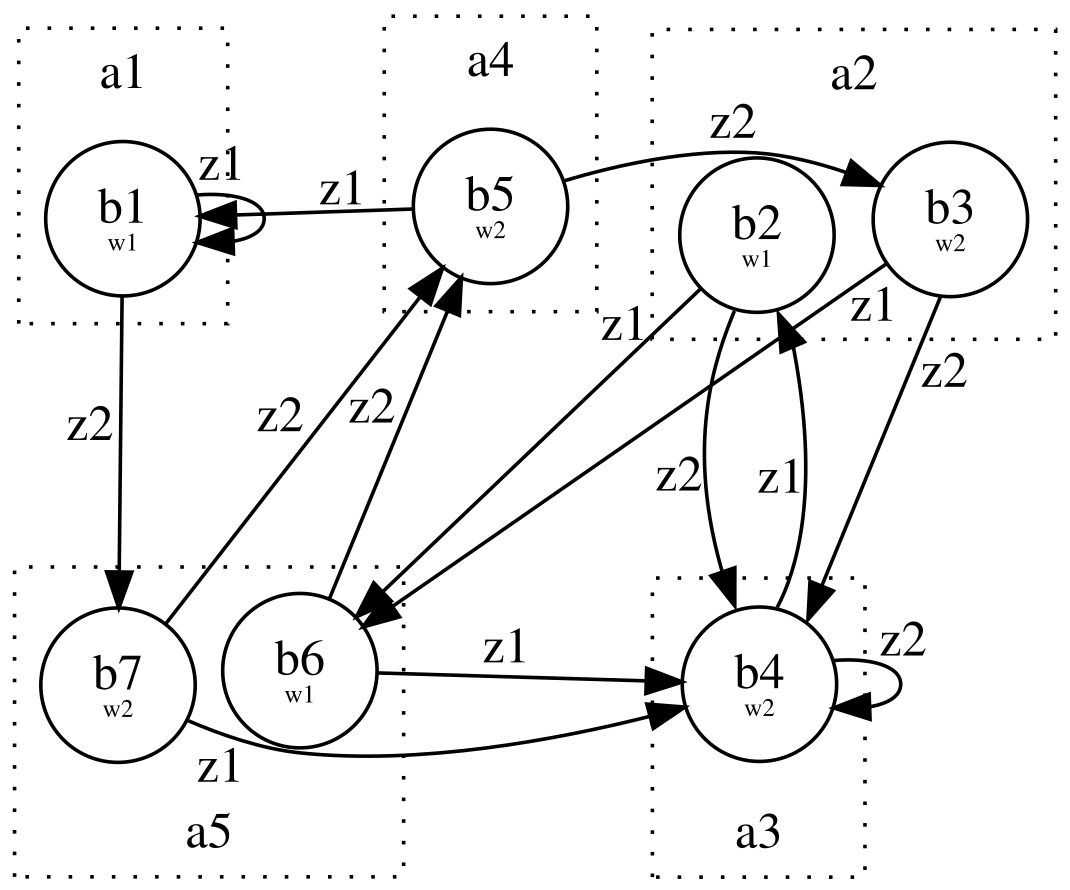
\includegraphics[width=0.5\textwidth]{moore.png}

\subsection*{Проверка на эквивалентность}

Рассмотрим входное слово, использованное для исходного автомата:

\begin{table}[h]
\begin{tabular}{|c|c|c|c|c|c|c|c|c|c|c|c|c|c|}
\hline
$z_1$ & $z_2$ & $z_1$ & $z_2$ & $z_1$ & $z_2$ & $z_1$ & $z_1$ & $z_2$ & $z_1$ & $z_2$ & $z_2$ & $z_2$ & \\\hline

$b_1$ & $b_1$ & $b_7$ & $b_4$ & $b_4$ & $b_2$ & $b_4$ & $b_2$ & $b_6$ & $b_5$ & $b_1$ & $b_7$ & $b_5$ & $b_3$ \\\hline

      & $w_1$ & $w_2$ & $w_2$ & $w_2$ & $w_1$ & $w_2$ & $w_1$ & $w_1$ & $w_2$ & $w_1$ & $w_2$ & $w_2$ & $w_2$ \\\hline
\end{tabular}
\caption{Поведение преобразованного автомата Мура}
\end{table}

Сравнивая с таблицей 1, можно увидеть, что выходные слова $w$ совпадают с задержкой на один такт, связанной с особенностью поведения автомата Мура, что позволяет утверждать об эквивалентности автоматов.

\section*{Обратное преобразование}

При переходе от автомата Мура к автомату Мили множество состояний и функции переходов совпадают, а функции выхода изменяются путем перемещения выходных сигналов из вершин (состояний) в дуги (переходы): 

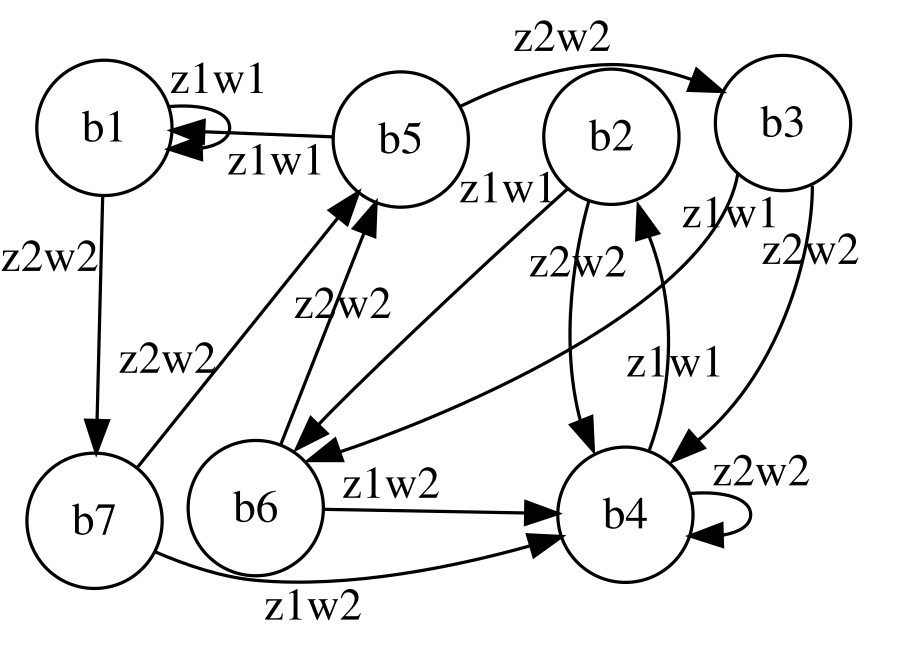
\includegraphics[width=0.5\textwidth]{mealy.png}

\subsection*{Проверка на эквивалентность}

Рассмотрим входное слово, использованное для исходного автомата:

\begin{table}[h]
\begin{tabular}{|c|c|c|c|c|c|c|c|c|c|c|c|c|c|}
\hline
$z_1$ & $z_2$ & $z_1$ & $z_2$ & $z_1$ & $z_2$ & $z_1$ & $z_1$ & $z_2$ & $z_1$ & $z_2$ & $z_2$ & $z_2$ & \\\hline

$b_1$ & $b_1$ & $b_7$ & $b_4$ & $b_4$ & $b_2$ & $b_4$ & $b_2$ & $b_6$ & $b_5$ & $b_1$ & $b_7$ & $b_5$ & $b_3$ \\\hline

$w_1$ & $w_2$ & $w_2$ & $w_2$ & $w_1$ & $w_2$ & $w_1$ & $w_1$ & $w_2$ & $w_1$ & $w_2$ & $w_2$ & $w_2$ & \\\hline
\end{tabular}
\caption{Поведение преобразованного автомата Мили}
\end{table}

Сравнивая с таблицей 1, можно увидеть, что выходные слова полностью совпадают, следовательно, автоматы эквивалентны. Такой же вывод можно сделать, рассмотрев таблицу 2 (с учетом задержки у автомата Мура).

\section*{Вывод}

В ходе выполнения работы были изучены отличия автомата Мура от автомата Мили, а также способы преобразования автомата Мили в автомат Мура и наоборот. При проверке преобразованных автоматов на эквивалентность было замечено, что реакция на входное слово автомата Мура задерживается на один такт по сравнению с автоматом Мили.

Стоит отметь, что автомат Мили, полученный из автомата Мура, обладает большим количеством состояний по сравнению с исходным автоматом Мили, хотя и является эквивалентным ему по свойству транзитивности.

\end{document}
